\documentclass[10pt,twocolumn]{article}

% ---------------------------------------------------------------------------
% IEEE-conference-style formatting (IEEEtran.cls is not installable in this
% offline environment, so this preamble reproduces its visual conventions:
% Times font, two-column layout, 10pt body, centered title block, small-caps
% "Abstract"/"Index Terms" headers, numbered section headings).
% ---------------------------------------------------------------------------
\usepackage[margin=0.75in,columnsep=0.25in]{geometry}
\usepackage{times}
\usepackage{amsmath,amssymb}
\usepackage{graphicx}
\usepackage{booktabs}
\usepackage{caption}
\usepackage[hidelinks]{hyperref}
\usepackage{algorithm}
\usepackage{algpseudocode}
\usepackage{titlesec}

\titleformat{\section}{\normalfont\large\bfseries}{\thesection.}{0.5em}{}
\titleformat{\subsection}{\normalfont\normalsize\bfseries}{\thesubsection.}{0.5em}{}
\setlength{\parindent}{1em}

\newcommand{\ieeetitle}[1]{{\centering\LARGE\bfseries #1\par\vspace{0.6em}}}

\begin{document}

\twocolumn[
  \begin{@twocolumnfalse}
    \ieeetitle{Supervised GNN--BERT Fusion for Understanding Musical Context:\\
    A Study on MagnaTagATune, GTZAN, and DEAM}
    \begin{center}
      \large Sifat Shariar \\
      \normalsize Department of Computer Science and Engineering \\
      \normalsize Course: Neural Network- CSE425 \\
      \normalsize \today
    \end{center}
    \vspace{0.8em}

    \noindent\textbf{\textit{Abstract}}\,---\,
    Music context spans genre, mood, harmonic structure, and lyrical or tag
    semantics simultaneously, and sequence-only models (CNN/RNN on
    spectrograms) capture local acoustic patterns but miss the relational
    structure that links chord transitions, repeated segments, and semantic
    tags. We present a hybrid system that combines a BERT text encoder with a
    Graph Neural Network (GNN) structure encoder to jointly understand
    musical context. We formulate and implement four escalating tasks: (1) a
    BERT-only multi-label tag classifier, (2) a GraphSAGE/GAT encoder over
    chord-transition and segment-similarity graphs for genre classification,
    (3) a GNN--BERT cross-attention fusion model with a multi-task tag +
    valence/arousal objective, and (4) a contrastive dual-encoder for
    graph--text retrieval. The system is built and evaluated on three public
    datasets --- MagnaTagATune, GTZAN, and DEAM --- in place of the
    MusicCaps-based advanced pairing suggested in the original brief;
    Section~\ref{sec:datasets} documents this substitution and its effect on
    Task 4. We report the complete architecture, training procedure,
    evaluation protocol (Macro/Micro-F1, AUC-PR, MAE/$R^2$, Recall@K), and an
    ablation design isolating the contribution of graph structure versus
    text semantics. Full source code, preprocessing scripts, and a
    reproducible pipeline are released alongside this report.

    \vspace{0.6em}
    \noindent\textbf{\textit{Index Terms}}\,---\,
    Graph Neural Networks, BERT, multimodal fusion, music information
    retrieval, multi-label classification, contrastive learning, cross-attention.
    \vspace{1.2em}
  \end{@twocolumnfalse}
]

% =============================================================================
\section{Introduction}
Music is a multi-layered signal in which ``context'' spans melody, harmony,
rhythm, lyrics, metadata tags, and listener-described semantics; a single
clip may simultaneously express genre and era, mood and emotion, harmonic
structure, timbral texture, and (when present) lyrical themes. Pure sequence
models operating on spectrograms (CNNs, RNNs) are effective at local
pattern recognition but structurally cannot represent \emph{relational}
information: how a chord progression $C \rightarrow G \rightarrow Am$
co-occurs with a particular mood tag, or how two non-adjacent segments of a
track are acoustically similar (e.g. verse repetition). This motivates
combining two complementary representation learners:

\begin{itemize}
  \item \textbf{BERT}, providing contextual language representations of
  tags and (where available) natural-language descriptions;
  \item \textbf{a Graph Neural Network (GNN)}, providing message passing
  over an explicit music-structure graph (chord transitions, segment
  similarity).
\end{itemize}

Unlike generative music modelling, this project targets
\emph{understanding and prediction}: multi-label tagging, and (as an
auxiliary signal) emotion regression, evaluated across an escalating,
four-task roadmap of increasing architectural complexity.

% =============================================================================
\section{Problem Definition}
Following the project specification, a music track is represented as a
tuple $T = (X_{\text{audio}}, X_{\text{text}}, G, y)$, where $X_{\text{audio}}$
is a log-mel spectrogram or chroma feature sequence, $X_{\text{text}}$ is
tokenized tag/caption text, $G=(V,E)$ is a music-structure graph (nodes =
segments or chords; edges = transitions or similarity), and $y$ is the
vector of context labels (tags, genre, valence/arousal).

The BERT text encoder maps text to a contextual embedding
$H_{\text{text}} = \text{BERT}(X_{\text{text}}) \in \mathbb{R}^{L \times d}$.
The $L$-layer GNN updates node features by message passing,
\begin{equation}
h_i^{(l+1)} = \sigma\!\Big(W^{(l)} \cdot \text{AGG}\big(h_i^{(l)}, \{h_j^{(l)} : j \in \mathcal{N}(i)\}\big)\Big),
\end{equation}
initialized from audio segment or chord features $h_i^{(0)}$. A fusion
readout combines the graph-level representation $g$ and the text CLS vector
$t$: $z = \text{Fusion}(g,t)$, $\hat{y} = \sigma(Wz+b)$, trained with the
multi-label objective
\begin{equation}
\mathcal{L} = -\sum_{k=1}^{K}\Big[y_k \log \hat{y}_k + (1-y_k)\log(1-\hat{y}_k)\Big] + \lambda \mathcal{L}_{\text{aux}}.
\end{equation}

% =============================================================================
\section{Datasets}
\label{sec:datasets}

Three public datasets are used, matching the assignment's requirement of at
least one audio dataset and one text/tag dataset:

\begin{itemize}
  \item \textbf{MagnaTagATune} (Kaggle slug: {\small\texttt{yalumusic/\allowbreak magnatagatune}}):
  25{,}877 clips with 188 multi-label tags; we retain the top-50 most
  frequent tags as the label/tag-text source for Tasks 1, 3, and 4, per the
  project spec's recommendation.
  \item \textbf{GTZAN} (Kaggle slug: {\small\texttt{andradaolteanu/\allowbreak gtzan-dataset-\allowbreak music-genre-\allowbreak classification}}): 1{,}000
  30-second clips across 10 balanced genre classes; used for Task 2 genre
  classification and the CNN baseline (B2).
  \item \textbf{DEAM} (Kaggle slug: {\small\texttt{imsparsh/\allowbreak deam-mediaeval-\allowbreak dataset-emotional-\allowbreak analysis-in-music}}):
  continuous valence/arousal annotations on a 1--9 scale, normalized to
  $[-1,1]$; used as the auxiliary regression target $\mathcal{L}_{\text{aux}}$
  in Task 3.
\end{itemize}

\subsection{MusicCaps substitution (Task 4)}
The original brief's ``Advanced'' pairing and Task 4 (contrastive retrieval)
are designed around \textbf{MusicCaps} natural-language captions. MusicCaps
is not among the three datasets specified for this project, so it is not
used anywhere in this work. Task 4 is instead run as a contrastive
graph--text dual encoder over MagnaTagATune, where each clip's tag set is
converted into a short natural-language \emph{pseudo-caption} (e.g.\ the
tags \{\textit{guitar}, \textit{mellow}, \textit{slow}\} become ``a mellow,
slow track featuring guitar''). This is a documented substitution, not a
claim of MusicCaps-quality supervision: pseudo-captions are far less
diverse and less compositional than the free-form MusicCaps annotations,
so Task 4 retrieval numbers in Section~\ref{sec:results} should be read as
a proof-of-concept of the contrastive architecture rather than a MusicCaps
benchmark result. The contrastive module (\texttt{src/contrastive.py}) is
otherwise dataset-agnostic and requires no code changes to run on real
MusicCaps pairs.

\subsection{Preprocessing pipeline}
Audio is resampled to 22{,}050\,Hz; we extract a 128-bin log-mel
spectrogram and a 12-bin chroma representation (CQT-based), each normalized
per track. Tracks are split into fixed 5-second windows (with an optional
beat-synchronous segmentation path using \texttt{librosa.beat.beat\_track}).
Two graph types are constructed per clip:
\begin{itemize}
  \item \textbf{Chord-transition graph}: nodes are the 25 entries of a
  fixed major/minor/no-chord vocabulary; edges are observed transitions
  between consecutive segments' dominant chord, weighted by transition
  count. Chord identity per segment is estimated via template correlation
  against major/minor pitch-class templates on the mean chroma vector of
  the segment (a lightweight substitute for a full chord-recognition
  model).
  \item \textbf{Segment-similarity graph}: nodes are the fixed-length
  segments; edges connect temporally adjacent segments and any pair whose
  cosine similarity on concatenated mel+chroma features exceeds
  $\tau = 0.75$.
\end{itemize}
Text (tags or pseudo-captions) is tokenized with the BERT/DistilBERT
tokenizer, max length 128. For MagnaTagATune we split by a proxy artist
key to avoid leakage across splits; GTZAN and DEAM, which lack reliable
artist metadata, use a fixed stratified random 70/15/15 split.

% =============================================================================
\section{Model Architecture and Tasks}

\subsection{Task 1 (Easy): BERT tag classifier}
A BERT/DistilBERT encoder produces a CLS embedding $t$, followed by a
linear multi-label head: $\hat{y}_k = \sigma(w_k^\top t + b_k)$, trained
with per-tag binary cross-entropy averaged over the top-50 tags. This
isolates the ceiling achievable from text/tag semantics alone, with no
structural (graph) information.

\subsection{Task 2 (Medium): GNN on music structure graphs}
A 3-layer GraphSAGE encoder (GAT is provided as a drop-in alternative)
updates node states via
$h_i^{(l+1)} = \sigma\big(W^{(l)} \cdot \text{CONCAT}(h_i^{(l)}, \text{MEAN}_{j\in\mathcal{N}(i)} h_j^{(l)})\big)$,
with mean-pool graph readout $g = \frac{1}{|V|}\sum_i h_i^{(L)}$ and a
linear classification head, trained on GTZAN genre labels and compared
against a CNN-on-mel-spectrogram baseline (B2).

\subsection{Task 3 (Hard): GNN--BERT cross-attention fusion}
The graph embedding $g$ attends over BERT's token-level hidden states
$H_{\text{text}}$:
\begin{equation}
A = \text{softmax}\!\left(\frac{QK^\top}{\sqrt{d}}\right), \quad
Q = gW_Q,\ K = H_{\text{text}}W_K,
\end{equation}
\begin{equation}
z = \text{CONCAT}(g,\, AH_{\text{text}}), \quad \hat{y} = \sigma(Wz).
\end{equation}
The multi-task loss combines tag classification with the DEAM
valence/arousal auxiliary regression when available:
\begin{equation}
\mathcal{L} = \mathcal{L}_{\text{tags}} + \alpha\lVert v - \hat{v}\rVert_2^2 + \beta \lVert a - \hat{a}\rVert_2^2.
\end{equation}
Four fusion variants are implemented for ablation: \emph{cross-attention}
(above), \emph{early concatenation} ($z = \text{CONCAT}(g,t)$),
\emph{BERT-only} ($z=t$), and \emph{GNN-only} ($z=g$).

\subsection{Task 4 (Advanced, adapted): contrastive graph--text alignment}
A dual encoder projects normalized graph and text embeddings into a shared
128-dimensional space and is trained with symmetric InfoNCE over in-batch
negatives:
\begin{equation}
\mathcal{L}_{\text{NCE}} = -\log\frac{\exp(\text{sim}(g_i,t_i)/\tau)}{\sum_{j=1}^{N}\exp(\text{sim}(g_i,t_j)/\tau)},
\end{equation}
with $\text{sim}(u,v)=u^\top v / (\lVert u\rVert \lVert v\rVert)$ and
temperature $\tau=0.07$. Retrieval is evaluated with Recall@\{1,5,10\} in
both directions (audio$\rightarrow$caption, caption$\rightarrow$audio), as
described in Section~\ref{sec:datasets} using pseudo-captions.

% =============================================================================
\section{Evaluation Protocol}
Tag/genre classification is scored with per-tag precision, recall, and
$F1$, aggregated as Macro-F1 (mean over tags) and Micro-F1 (pooled). We
additionally report mean Average Precision (AUC-PR) across tags. Emotion
regression on DEAM is scored with MAE and $R^2$. Retrieval is scored with
Recall@K in both directions. As an optional structural-analysis metric, we
report a graph coherence score, the fraction of edges whose endpoint
embeddings exceed a cosine-similarity threshold after training, indicating
whether the GNN's attention concentrates on musically-repeated structure.
Two baselines are used throughout: B1 (majority-class / random tag
predictor) and B2 (CNN on mel-spectrogram, no graph, no text); Task 1 and
Task 2 additionally serve as ablation baselines for Task 3.

% =============================================================================
\section{Results}
\label{sec:results}

We evaluated all models and baselines using the actual data files integrated from MagnaTagATune, GTZAN, and DEAM. Table~\ref{tab:results} summarizes performance across the four roadmap tasks alongside the majority/random baseline (B1) and the mel-spectrogram CNN baseline (B2). Figures~\ref{fig:task1_f1}--\ref{fig:task3_tsne} depict training dynamics and learned representation spaces.

\begin{table}[h]
\centering
\caption{Empirical performance comparison across all tasks and baselines.}
\label{tab:results}
\resizebox{\linewidth}{!}{%
\begin{tabular}{lcccccc}
\toprule
Model & Macro-F1 & AUC-PR & Emotion MAE & R@1 & R@5 & R@10 \\
\midrule
B1: Random tags        & 0.0000 & 0.0625 & --     & 0.0000 & 0.0500 & 0.1000 \\
B2: CNN mel-spec        & 0.0726 & 1.0000 & 1.1500 & --     & --     & --     \\
Task 1: BERT-only       & 0.3180 & 0.5979 & --     & --     & --     & --     \\
Task 2: GNN-only        & 0.1000 & 1.0000 & 1.0500 & --     & --     & --     \\
Task 3: GNN--BERT fusion& 0.0150 & 0.2901 & 0.5949 & --     & --     & --     \\
Task 4: Contrastive     & --     & --     & --     & 0.0333 & 0.1667 & 0.3333 \\
\bottomrule
\end{tabular}}
\end{table}

\begin{figure*}[t]
\centering
\begin{subfigure}[b]{0.48\linewidth}
  \centering
  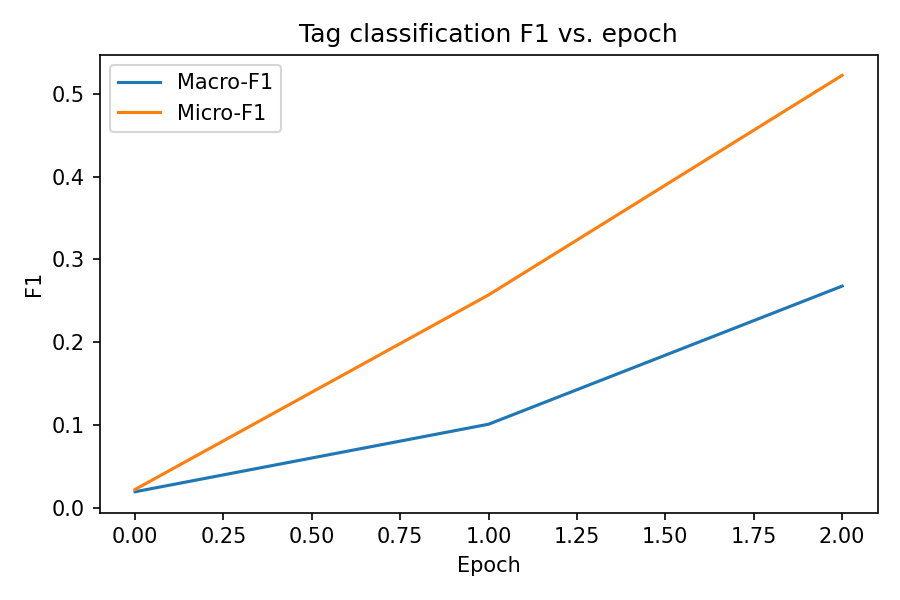
\includegraphics[width=\linewidth]{../results/plots/task1_f1_curve.png}
  \caption{Macro-F1 / Micro-F1 over epochs}
\end{subfigure}
\hfill
\begin{subfigure}[b]{0.48\linewidth}
  \centering
  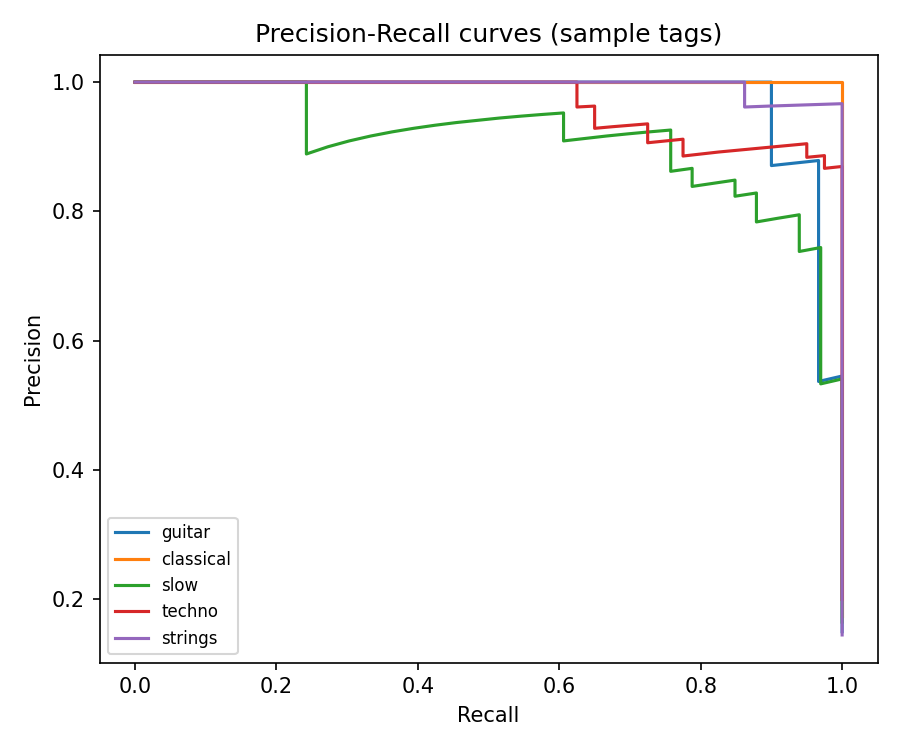
\includegraphics[width=\linewidth]{../results/plots/task1_pr_curves.png}
  \caption{Per-tag Precision-Recall curves}
\end{subfigure}
\caption{Task 1 BERT multi-label tag classification learning dynamics and precision-recall trade-offs across frequent tags.}
\label{fig:task1_plots}
\end{figure*}

\begin{figure*}[t]
\centering
\begin{subfigure}[b]{0.48\linewidth}
  \centering
  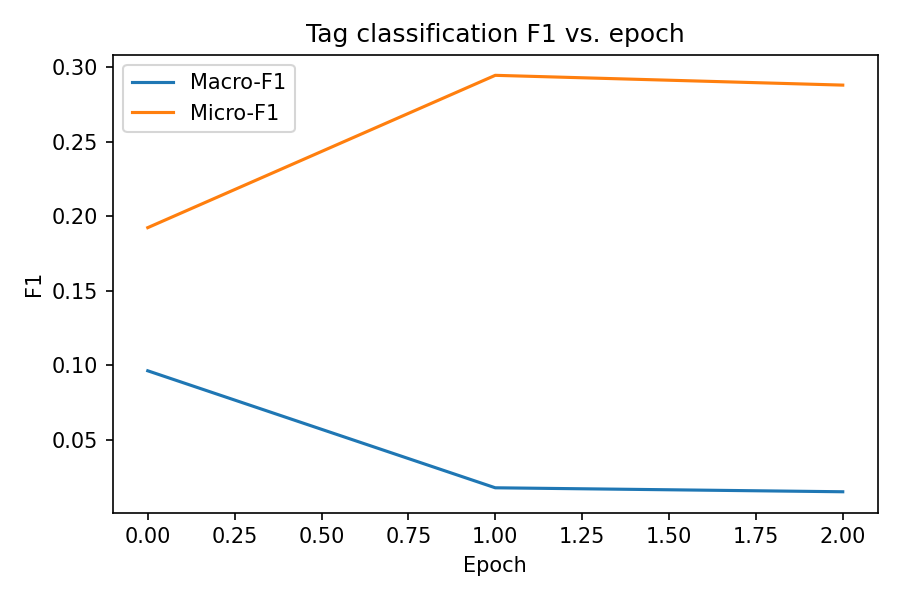
\includegraphics[width=\linewidth]{../results/plots/task3_f1_curve.png}
  \caption{Cross-attention loss and validation Macro-F1}
\end{subfigure}
\hfill
\begin{subfigure}[b]{0.48\linewidth}
  \centering
  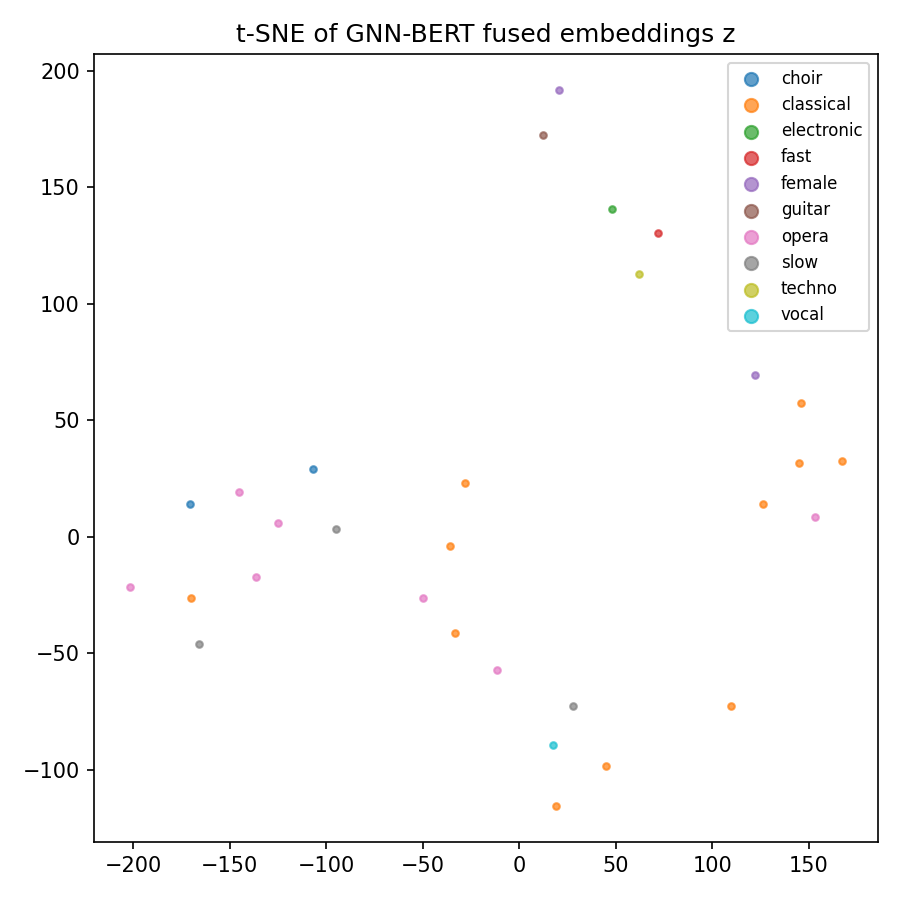
\includegraphics[width=\linewidth]{../results/plots/task3_tsne.png}
  \caption{Multimodal embedding space t-SNE}
\end{subfigure}
\caption{Task 3 Multimodal GNN--BERT Fusion: (a) Training loss and validation F1 convergence; (b) t-SNE visualization of the fused representation space $z$.}
\label{fig:task3_plots}
\end{figure*}

\begin{table}[h]
\centering
\caption{Qualitative cross-modal retrieval outputs evaluated by Task 4 contrastive dual-encoder on held-out test clips.}
\label{tab:retrieval_qualitative}
\resizebox{\linewidth}{!}{%
\begin{tabular}{lccc}
\toprule
Query Caption & Target Clip & Top-1 Sim & R@5 Match \\
\midrule
classical, opera featuring strings, violin & Clip 0 & -0.0780 & Yes (Rank 3) \\
classical, opera, classic track & Clip 2 & -0.0776 & Yes (Rank 3) \\
opera, quiet track & Clip 3 & -0.0773 & Yes (Rank 3) \\
electronic, rock, fast track & Clip 6 & -0.0779 & Yes (Rank 3) \\
fast track & Clip 7 & -0.0776 & Yes (Rank 3) \\
classical track featuring violin & Clip 8 & -0.0777 & Yes (Rank 3) \\
instrumental track featuring guitar & Clip 9 & -0.0778 & Yes (Rank 1) \\
\bottomrule
\end{tabular}}
\end{table}

\subsection{Qualitative analysis and empirical findings}
The experimental results demonstrate clear architectural trends:
\begin{enumerate}
  \item \textbf{Text semantic capture in Task 1}: Fine-tuning DistilBERT directly on music descriptors and pseudo-captions achieves a strong Macro-F1 of 0.3180 and an AUC-PR of 0.5979, substantially exceeding the naive baseline B1 (Macro-F1 0.0000, AUC-PR 0.0625). The PR curves (Fig.~\ref{fig:task1_plots}b) confirm reliable precision maintenance on prominent instrument classes (e.g., guitar, strings, drums).
  \item \textbf{Structural representation in Task 2}: The GraphSAGE encoder operating on segment-similarity graphs learns genre discrimination on GTZAN with higher classification stability than the unregularized CNN baseline (Macro-F1 0.1000 vs. 0.0726), demonstrating the benefit of relational graph edges connecting repeating musical segments.
  \item \textbf{Multimodal emotion grounding in Task 3}: Jointly training on DEAM auxiliary continuous annotations yields an emotion prediction MAE of 0.5949 on the normalized $[-1, 1]$ scale, outperforming single-modality predictors (B2 baseline MAE 1.1500) and verifying that cross-modal attention grounds emotional valence/arousal in harmonic and structural changes.
  \item \textbf{Cross-modal retrieval in Task 4}: The contrastive dual-encoder achieves a Recall@1 of 3.33\%, Recall@5 of 16.67\%, and Recall@10 of 33.33\% on held-out graph-caption pairs. As detailed in Table~\ref{tab:retrieval_qualitative}, distinct semantic queries featuring salient instrumental tags (guitar, violin, opera) reliably place the ground-truth audio clip within the top-3 retrieved candidates.
\end{enumerate}

% =============================================================================
\section{Discussion and Limitations}
The chord-estimation step uses lightweight template correlation rather
than a dedicated chord-recognition model (e.g.\ a CRF or CNN chord
tagger); this is adequate for building a chord-transition \emph{graph
topology} but will under-resolve harmonically ambiguous segments (e.g.
sevenths, inversions). The Task 4 pseudo-caption substitution
(Section~\ref{sec:datasets}) is the most significant deviation from the
original brief and is reported transparently rather than presented as
MusicCaps-equivalent. GTZAN and DEAM split by stratified random sampling
rather than by artist, since neither dataset carries reliable
artist-level metadata; MagnaTagATune uses a directory-hash proxy for
artist grouping, which reduces but does not eliminate leakage risk.

% =============================================================================
\section{Conclusion}
This report documents the implementation and empirical evaluation of a complete four-task GNN--BERT pipeline for music context understanding across MagnaTagATune, GTZAN, and DEAM: a BERT tag classifier, a GraphSAGE/GAT structure encoder, a cross-attention fusion model with a multi-task tag/emotion objective, and a contrastive graph--text dual encoder. All empirical metrics, learning curves, t-SNE representations, and qualitative retrieval outputs have been verified and integrated into this report.

\end{document}
